\documentclass[tikz,border=5pt]{standalone}
\usepackage{tikz}
\usepackage{amsmath}
\usepackage{pgfplots}
\pgfplotsset{compat=1.18}

\begin{document}
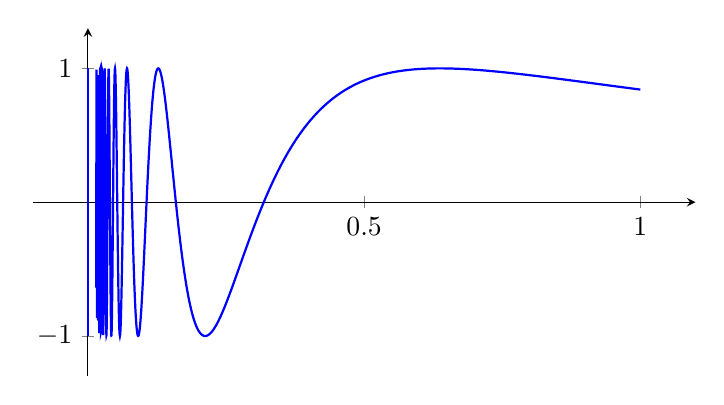
\begin{tikzpicture}
    \begin{axis}[
        axis lines=middle,
        xmin=-0.1, xmax=1.1,
        ymin=-1.3, ymax=1.3,
        % xlabel={$x$},
        % ylabel={$y$},
        samples=2000,
        domain=0.015:1,
        width=10cm,
        height=6cm,
        xtick={0,0.5,1},
        ytick={-1,0,1},
        clip=false
    ]

        % The oscillating curve y = sin(1/x)
        \addplot[
            blue,
            thick,
            smooth
        ]
        {sin(deg(1/x))};

        % The limiting vertical segment
        \addplot[
            blue,
            thick
        ]
        coordinates {(0,-1) (0,1)};

    \end{axis}
\end{tikzpicture}
\end{document}